\documentclass[a4paper]{article}
\usepackage[normalem]{ulem}
\usepackage{eurosym}
\usepackage[font=small,labelfont=bf]{caption}
\usepackage{graphicx}

% impostazioni generali
%Tutti gli usepackage vanno qui
\usepackage{geometry}
\usepackage[italian]{babel}
\usepackage[utf8]{inputenc}
\usepackage{tabularx}
\usepackage{longtable}
\usepackage{hyperref}
\usepackage{enumitem}
\usepackage{array} 
\usepackage{booktabs}
\newcolumntype{M}[1]{>{\centering\arraybackslash}m{#1}}
\usepackage[toc]{appendix}

\hypersetup{
	colorlinks=true,
	linkcolor=blue,
	filecolor=magenta,
	urlcolor=blue,
}
% Numerazione figure
\let\counterwithout\relax
\let\counterwithin\relax
\usepackage{chngcntr}

% distanziare elenco delle figure e delle tabelle
\usepackage{tocbasic}
\DeclareTOCStyleEntry[numwidth=3.5em]{tocline}{figure}% for figure entries
\DeclareTOCStyleEntry[numwidth=3.5em]{tocline}{table}% for table entries


\counterwithin{table}{subsection}
\counterwithin{figure}{subsection}

\usepackage[bottom]{footmisc}
\usepackage{fancyhdr}
\setcounter{secnumdepth}{4}
\usepackage{amsmath, amssymb}
\usepackage{array}
\usepackage{graphicx}

\usepackage{ifthen}

\usepackage{float}
\restylefloat{table}

\usepackage{layouts}
\usepackage{url}
\usepackage{comment}
\usepackage{eurosym}

\usepackage{lastpage}
\usepackage{layouts}
\usepackage{eurosym}

\geometry{a4paper,top=3cm,bottom=4cm,left=2.5cm,right=2.5cm}

%Comandi di impaginazione uguale per tutti i documenti
\pagestyle{fancy}
\lhead{
\includegraphics[scale=0.1]{../../../template/images/logo_no_motto.jpeg}}
%Titolo del documento
\rhead{\doctitle{}}
%\rfoot{\thepage}
\cfoot{Pagina \thepage\ di \pageref{LastPage}}
\setlength{\headheight}{35pt}
\setcounter{tocdepth}{5}
\setcounter{secnumdepth}{5}
\renewcommand{\footrulewidth}{0.4pt}

% multirow per tabelle
\usepackage{multirow}

% Permette tabelle su più pagine
%\usepackage{longtable}


% colore di sfondo per le celle
\usepackage[table]{xcolor}

%COMANDI TABELLE
\newcommand{\rowcolorhead}{\rowcolor[HTML]{007c95}}
\newcommand{\cellcolorhead}{\cellcolor[HTML]{007c95}}
\newcommand{\hlinetable}{\arrayrulecolor[HTML]{007c95}\hline}

%intestazione
% check for missing commands
\newcommand{\headertitle}[1]{\textbf{\color{white}#1}} %titolo colonna
\definecolor{pari}{HTML}{b1dae3}
\definecolor{dispari}{HTML}{d7f2f7}

% comandi glossario
\newcommand{\glo}{$_{G}$}
\newcommand{\glosp}{$_{G}$ }


%label custom
\makeatletter
\newcommand{\uclabel}[2]{%
	\protected@write \@auxout {}{\string \newlabel {#1}{{#2}{\thepage}{#2}{#1}{}} }%
	\hypertarget{#1}{#2}
}
\makeatother

%riportare pezzi di codice
\definecolor{codegray}{gray}{0.9}
\newcommand{\code}[1]{\colorbox{codegray}{\texttt{#1}}}



% dati relativi alla prima pagina
% Configurazione della pagina iniziale
\newcommand{\doctitle}{\textit{Verbale} interno 01-12-2022 }
\newcommand{\docdate}{01 Dicembre 2022}
\newcommand{\rev}{1.0.0}
\newcommand{\stato}{Approvato}
\newcommand{\uso}{Interno}
\newcommand{\approv}{Elena Pandolfo}
\newcommand{\red}{Tommaso Allegretti}
\newcommand{\ver}{Gabriele Mantoan\\& Mirko Stella}
\newcommand{\dest}{\textit{Seven Clickers}
									  \\ Prof. Vardanega Tullio 
									   \\ Prof. Cardin Riccardo}
\newcommand{\describedoc}{\textit{Verbale} riguardante il meeting tenuto il giorno 01-12-2022}


 % editare questo

\makeindex

\begin{document}
\counterwithin{table}{section}

% Prima pagina
\thispagestyle{empty}
\renewcommand{\arraystretch}{1.3}

\begin{titlepage}
	\begin{center}
		
	
\includegraphics[scale = 0.40]{../../../template/images/logo.jpeg}
	\\[1cm]
	\href{mailto:7clickersgroup@gmail.com}		      	
	{\large{\textit{7clickersgroup@gmail.com} } }\\[2.5cm]
	\Huge \textbf{\doctitle} \\[1cm]
	 \large
			 \begin{tabular}{r|l}
                        \textbf{Versione} & \rev{} \\
                        \textbf{Stato} & \stato{} \\
                        \textbf{Uso} & \uso{} \\                         
                        \textbf{Approvazione} & \approv{} \\                      
                        \textbf{Redazione} & \red{} \\ 
                        \textbf{Verifica} &  \ver{} \\                         
                        \textbf{Distribuzione} & \parbox[t]{5cm}{ \dest{} }
                \end{tabular} 
                \\[3.5cm]
                \large \textbf{Descrizione} \\ \describedoc{} 
     \end{center}
\end{titlepage}

% Diario delle modifiche
\section*{Registro delle modifiche}

\newcommand{\changelogTable}[1]{
	 

\renewcommand{\arraystretch}{1.5}
\rowcolors{2}{pari}{dispari}
\begin{longtable}{ 
		>{\centering}M{0.07\textwidth} 
		>{\centering}M{0.13\textwidth}
		>{\centering}M{0.20\textwidth}
		>{\centering}M{0.17\textwidth} 
		>{\centering\arraybackslash}M{0.30\textwidth} 
		 }
	\rowcolorhead
	\headertitle{Vers.} &
	\centering \headertitle{Data} &	
	\headertitle{Autore} &
	\headertitle{Ruolo} & 
	\headertitle{Descrizione} 
	\endfirsthead	
	\endhead
	
	#1

\end{longtable}
\vspace{-2em}

}



\changelogTable{
	1.0.0 & 14-12-22 & Elena Pandolfo & Responsabile &  Approvazione documento\tabularnewline
	0.1.0 & 01-12-22 & Gabriele Mantoan \\ Mirko Stella & Verificatori & Verifica documento\tabularnewline
	0.0.1 & 09-11-22 & Rino Sincic & Analista &  Redazione documento\\
} % editare questo
\pagebreak

% Indice
{
    \hypersetup{linkcolor=black}
    \tableofcontents
    \listoffigures
}
\pagebreak

% Contenuto
\section{Introduzione}
\subsection{Scopo del documento}
Questo documento è stato creato dal gruppo Seven Clickers per descrivere degli standard fissati e dei metodi utilizzati al fine di garantire la qualità dei prodotti e dei processi.
In questo documento vengono tracciati periodicamente i risultati ottenuti che verranno analizzati tramite misurazioni permettendoci di correggere eventuali problematiche.

\subsection{Scopo del capitolato}
Il capitolato su cui noi Seven Clickers lavoriamo nasce da una proposta dell'azienda SanMarco Informatica per evitare sprechi dovuti all'utilizzo di uno ShowRoom tradizionale proponendo uno ShowRoom 3D con un ambientazione ugualmente o più coinvolgente.

\subsection{Glossario}
In questo documento sono state segnate con il pedice "g" tutte le parole che, secondo noi, necessitano di una loro definizione più accurata nel documento di \textit{Glossario}.

\subsection{Riferimenti}
\subsubsection{Riferimenti normativi}
\begin{itemize}
\item \textit{Norme di Progetto}.
\end{itemize}

\subsubsection{Riferimenti informativi}
\begin{itemize}
	\item Materiale didattico Ingegneria del Software - T02 Processi di ciclo di vita: \url{https://www.math.unipd.it/~tullio/IS-1/2022/Dispense/T02.pdf}
	\item Materiale didattico Ingegneria del Software - T08 Qualità di prodotto: \url{https://www.math.unipd.it/~tullio/IS-1/2022/Dispense/T08.pdf}
	\item Materiale didattico Ingegneria del Software - T09 Qualità di processo: \url{https://www.math.unipd.it/~tullio/IS-1/2022/Dispense/T09.pdf}
	\item Indice di Gulpease: \url{https://it.wikipedia.org/wiki/Indice_Gulpease}
	\item Complessità ciclomatica: \url{https://www.math.unipd.it/~tullio/IS-1/2022/Dispense/T12.pdf}
	\item Code coverage: \url{https://www.math.unipd.it/~tullio/IS-1/2022/Dispense/T12.pdf}	
	\item Lo standard ISO/IEC 12207:1995 : \url{https://www.math.unipd.it/~tullio/IS-1/2009/Approfondimenti/ISO_12207-1995.pdf}
	\item Riferimento per alcune metriche di processo: \url{https://it.wikipedia.org/wiki/Metriche_di_progetto}
	\item Requirements Stability Index (RSI): \\ \url{https://shiyamtj.wordpress.com/2018/09/26/requirement-stability-index/}
	\item Defect Density: \url{https://www.softwaretestinghelp.com/defect-density/}
\end{itemize}

\section{Qualità del processo}
Per mantenere la qualità dei processi il gruppo ha deciso di utilizzare lo standard \textbf{ISO/IEC 12207:1995} scegliendo i processi più adatti al nostro progetto, adeguandoli e semplificandoli in base alle necessità del progetto.

\subsection{Obiettivi di qualità del processo}
Nelle seguenti tabelle vengono identificati i processi, una loro breve descrizione e le metriche a loro associate. Viene utilizzato, per le metriche di qualità di processo, la denominazione MPC (Metrica processo) associata ad un numero che incrementa fino al numero di metriche utilizzate in questa sezione.
\subsubsection{Processi primari}
\begin{longtable}{ 
		>{\centering}M{0.20\textwidth} 
		>{\centering}M{0.50\textwidth}
		>{\centering}M{0.17\textwidth} 
		}
	\rowcolorhead
	\headertitle{Processo} &
	\centering \headertitle{Descrizione} &	
	\headertitle{Metriche} 
	\endfirsthead
	\endhead
	
	Fornitura & Processo dedito alla determinazione delle procedure e delle risorse necessarie per gestire e garantire il progetto. & MPC01, MPC02, MPC03, MP04, MPC05, MPC06, MPC07, MPC08\tabularnewline
	Sviluppo & Processo contenente le attività relative alle sviluppo del progetto & MPC09\tabularnewline
\end{longtable}

\subsubsection{Processi di supporto}
\begin{longtable}{ 
		>{\centering}M{0.20\textwidth} 
		>{\centering}M{0.50\textwidth}
		>{\centering}M{0.17\textwidth} 
		}
	\rowcolorhead
	\headertitle{Processo} &
	\centering \headertitle{Descrizione} &	
	\headertitle{Metriche} 
	\endfirsthead
	\endhead
	
	Documentazione & Processo dedicato al controllo dei documenti prodotti. I documenti prodotti devono essere leggibili e comprensibili a lettori con licenza media. & MPC10\tabularnewline
	Accertamento della qualità & Processo che garantisce la conformità dei processi e dei prodotti ai requisiti specificati e ai loro piani & MPC11\tabularnewline
	Verifica & Processo che determina se le condizioni o i requisiti di un prodotto sono soddisfatti. Questo processo include analisi,revisione e test & MPC12\tabularnewline	
\end{longtable}

\subsubsection{Processi organizzativi}
\begin{longtable}{ 
		>{\centering}M{0.20\textwidth} 
		>{\centering}M{0.50\textwidth}
		>{\centering}M{0.17\textwidth} 
		}
	\rowcolorhead
	\headertitle{Processo} &
	\centering \headertitle{Descrizione} &	
	\headertitle{Metriche} 
	\endfirsthead
	\endhead
	
	Gestione organizzativa & Processo che organizza,monitora e controlla le prestazioni di un processo & MPC13\tabularnewline	
\end{longtable}

\subsection{Metriche utilizzate}
\begin{longtable}{
		>{\centering}M{0.17\textwidth}
		>{\centering}M{0.20\textwidth}	 
		>{\centering}M{0.23\textwidth}
		>{\centering}M{0.24\textwidth} 
		}
	\rowcolorhead
	\headertitle{ID} &
	\centering \headertitle{Metrica} &	
	\headertitle{Valore minimo} &
	\headertitle{Valore ottimo} 
	\endfirsthead	
	\endhead
MPC01 & Planned Value (PV) & $ \ge 0 $ \euro & $ \le \text{Budget at Completion} $ \tabularnewline
MPC02 & Actual Cost (AC) & $ \ge 0 $ \euro & $ \le \text{EAC} $\tabularnewline
MPC03 & Earned Value (EV) & $ \ge 0 $ \euro & $ \le \text{EAC} $ \tabularnewline
MPC04 & Estimated at Completion (EAC) & preventivo -5\% $ \le \text{EAC} $ preventivo +5\% $ \ge \text{EAC} $   & Costo preventivato \tabularnewline
MPC05 & Estimated to Complete (ETC) & $ \ge 0 $ \euro & $ \le \text{EAC} $ \tabularnewline
MPC06 & Cost Variance (CV) & $ \ge 0$ \euro &  0 \euro \tabularnewline
MPC07 & Schedule Variance (SV) & $ \ge -15\% $ & $ 0\% $ \tabularnewline
MPC08 & Budget Variance (BV) & $ \ge 0 $ \euro & 0 \euro \tabularnewline
MPC09 & Requirements Stability Index (RSI) & 70\% & 100\%\tabularnewline
MPC10 & Indice di Gulpease &  $ \ge 50 $ & $ \ge 80 $\tabularnewline
MPC11 & Metriche soddisfatte & $ \ge 80\% $ & 100\% \tabularnewline
MPC12 & Code Coverage & $ \ge 70\% $  & $ \ge 90-100\% $\tabularnewline
MPC13 & Rischi non previsti & $\ge 0$ & 0 \tabularnewline
\end{longtable}

\section{Qualità del prodotto}
Il gruppo ha deciso di utilizzare lo standard \textbf{ISO/IEC 9126} selezionando le qualità necessarie per l'intero ciclo di vita del progetto selezionando delle metriche per il loro mantenimento.

\subsection{Obiettivi di qualità del prodotto}
Nelle seguenti tabelle vengono identificati gli obiettivi di qualità, una loro breve descrizione e le metriche a loro associate. Viene utilizzato, per le metriche di qualità di processo, la denominazione MPD (Metrica prodotto) associata ad un numero che incrementa fino al numero di metriche utilizzate in questa sezione.
\subsubsection{Software}
\begin{longtable}{ 
		>{\centering}M{0.20\textwidth} 
		>{\centering}M{0.50\textwidth}
		>{\centering}M{0.17\textwidth} 
		}
	\rowcolorhead
	\headertitle{Obiettivo} &
	\centering \headertitle{Descrizione} &	
	\headertitle{Metriche} 
	\endfirsthead	
	\endhead
	
	Funzionalità & Garantire con accuratezza e conformità le funzionalità poste nel documento di \textit{Analisi dei Requisiti} & MPD01\tabularnewline
	Affidabilità & Capacità del prodotto di svolgere le funzionalità implementate & MPD02\tabularnewline
	Efficienza & Mantenere una velocità di esecuzione del prodotto relativamente alle risorse utilizzate & MPD03,MPD04\tabularnewline
	Usabilità & Capacità del prodotto di essere utilizzato dall'utente & MPD05\tabularnewline
	Manutenibilità & Capacità di modificare il prodotto nel tempo & MPD06, MPD07\tabularnewline
	Portabilità & Capacità di funzionare in diversi ambienti di esecuzione & MPD08\tabularnewline
\end{longtable}

\subsection{Metriche utilizzate}
\begin{longtable}{
		>{\centering}M{0.17\textwidth}
		>{\centering}M{0.20\textwidth}	 
		>{\centering}M{0.23\textwidth}
		>{\centering}M{0.24\textwidth} 
		}
	\rowcolorhead
	\headertitle{ID} &
	\centering \headertitle{Metrica} &	
	\headertitle{Valore minimo} &
	\headertitle{Valore ottimo} 
	\endfirsthead	
	\endhead
MPD01 & Percentuale requisiti soddisfatti & 100\% requisiti obbligatori & 100\% tutti requisiti \tabularnewline
MPD02 & Densità fallimenti durante l'esecuzione & 20\% & 10\% \tabularnewline
MPD03 & Tempo medio di risposta & 4 secondi & 2 secondi \tabularnewline
MPD04 & Tempo di caricamento & 15 secondi & 10 secondi \tabularnewline
MPD05 & Facilità di apprendimento & 5 minuti & 2 minuti \tabularnewline
MPD06 & Complessità ciclomatica & $ \le 10 $ &  $ \le 4 $ \tabularnewline
MPD07 & Densità dei commenti & 20\% & 10\% \tabularnewline
MPD08 & Browser Supportati & 80\% & 100\% \tabularnewline
\end{longtable}

\section{Specifica dei Test}
\begin{itemize}
\item Test di unità: vengono stabiliti durante la progettazione e servono per verificare le singole unità software;
\item Test di integrazione: vengono stabiliti durante la progettazione e servono per integrare il funzionamento di più unità;
\item Test di accettazione: vengono effettuati insieme al proponente durante la fase di collaudo;
\item Test di sistema: vengono stabiliti durante l'analisi dei requisiti e servono per accertare la copertura dei requisiti software definiti nel documento di \textit{Analisi dei Requisiti}.
\end{itemize}
Gli acronimi utilizzati in questo documento per identificare i test sono specificati dettagliatamente nel documento di \textit{Norme di Progetto}.
In questa sezione vengono utilizzate le seguenti sigle per lo stato di ogni test:
\begin{itemize}
\item \textbf{S}: test superato
\item \textbf{N}: test non implementato
\end{itemize}

\subsection{Test di unità}
Questi test verranno stabiliti durante la Progettazione.

\subsection{Test di integrità}
Questi test verranno stabiliti durante la Progettazione.

\subsection{Test di accettazione}
Questi test verranno stabiliti durante la fase di Collaudo.

\subsection{Test di sistema}
Per assicurare che vengano rispettati i requisiti concordati nel documento di \textit{Analisi dei Requisiti}, vengono eseguiti i seguenti test di sistema.
\begin{longtable}{
		>{\centering}M{0.20\textwidth}
		>{\centering}M{0.35\textwidth}	 
		>{\centering}M{0.20\textwidth} 
		}
	\rowcolorhead
	\headertitle{Test} &
	\centering \headertitle{Descrizione} &	
	\headertitle{Stato} 
	\endfirsthead	
	\endhead
TSRF1 & Si verifica che l'utente possa aggiungere, l'oggetto con cui sta interagendo, nel carrello & N \tabularnewline
TSRF2 & Si verifica che l'utente possa visualizzare il contenuto del carrello & N \tabularnewline
TSRF2.1 & Si verifica che l'utente possa visualizzare la lista degli oggetti presenti nel carrello & N \tabularnewline
TSRF2.1.1 & Si verifica che l'utente possa interagire con un oggetto nel carrello & N \tabularnewline
TSRF2.1.1.1 & Si verifica che l'utente possa visualizzare la caratteristica del nome di ogni oggetto presente nella lista degli oggetti presenti nel carrello & N \tabularnewline
TSRF2.1.1.2 & Si verifica che l'utente possa visualizzare la caratteristica del costo di ogni oggetto presente nella lista degli oggetti presenti nel carrello & N \tabularnewline
TSRF2.1.1.3 & Si verifica che l'utente possa visualizzare la caratteristica della quantità di ogni oggetto presente nella lista degli oggetti presenti nel carrello & N \tabularnewline
TSRF2.2 & Si verifica che l'utente possa visualizzare il costo totale degli oggetti che ha inserito nel carrello & N \tabularnewline
TSRF3 & Si verifica che l'utente abbia la possibilità di rimuovere tutti gli oggetti dal carrello & N \tabularnewline
TSRF4 & Si verifica che l'utente abbia la possibilità di rimuovere un singolo oggetto dal carrello & N \tabularnewline
TSRF5 & Si verifica che l'utente possa muoversi in maniera direzionale & N \tabularnewline
TSRF5.1 & Si verifica che l'utente possa compiere movimenti direzionali nell'asse X & N \tabularnewline
TSRF5.2 & Si verifica che l'utente possa compiere movimenti direzionali nell'asse Y & N \tabularnewline
TSRF5.3 & Si verifica che l'utente possa compiere movimenti direzionali nell'asse Z & N \tabularnewline
TSRF6 & Si verifica che l'utente possa compiere spostamenti di camera & N \tabularnewline
TSRF6.1 & Si verifica che l'utente possa compiere spostamenti di camera nell'asse X & N \tabularnewline
TSRF6.2 & Si verifica che l'utente possa compiere spostamenti di camera nell'asse Y & N \tabularnewline
TSRF7 & Si verifica che l'utente possa modificare la combinazione dei colori di un oggetto & N \tabularnewline
TSRF8 & Si verifica che l'utente venga notificato in caso non fosse possibile modificare un oggetto & N \tabularnewline
TSRF9 & Si verifica che l'utente possa visualizzare la lista degli oggetti della stanza in cui si trova & N \tabularnewline
TSRF9.1 & Si verifica che l'utente possa visualizzare un singolo oggetto nella lista degli oggetti della stanza in cui si trova & N \tabularnewline
TSRF9.1.1 & Si verifica che l'utente possa visualizzare la caratteristica del nome di ogni oggetto della lista degli oggetti della stanza in cui si trova & N \tabularnewline
TSRF10 & Si verifica che l'utente possa visualizzare tutti i dettagli di un oggetto selezionato & N \tabularnewline
TSRF11 & Si verifica che l'utente abbia la possibilità di riposizionarsi vicino ad un oggetto nella stanza in cui si trova & N \tabularnewline
TSRF12 & Si verifica che l'utente possa riposizionarsi in una stanza da lui selezionata & N \tabularnewline
TSRF13 & Si verifica che l'utente venga notificato in caso il riposizionamento in una stanza non sia possibile & N \tabularnewline
TSRF14 & Si verifica che l'utente venga notificato in caso il riposizionamento in prossimità di un oggetto selezionato non sia concesso & N \tabularnewline
TSRF15 & Si verifica che l'utente possa visualizzare la lista delle stanze & N \tabularnewline
TSRF15.1 & Si verifica che l'utente possa visualizzare una singola stanza dalla lista delle stanze & N \tabularnewline
TSRF15.1.1 & Si verifica che l'utente possa visualizzare la caratteristica del nome di ogni stanza dalla lista delle stanze & N \tabularnewline
TSRF15.1.2 & Si verifica che l'utente possa visualizzare la caratteristica della tipologia di oggetti presenti in ogni stanza nella lista delle stanze & N \tabularnewline
TSRF16 & Si verifica che l'utente possa riposizionare un oggetto presente nella stanza in cui si trova & N \tabularnewline
TSRF17 & Si verifica che l'utente non possa riposizionare un oggetto in una coordinata non legittima & N \tabularnewline
TSRF18 & Si verifica che l'utente sia in grado ad illuminare l'ambiente davanti a lui & N \tabularnewline
TSRF19 & Si verifica che l'utente venga notificato se il contenuto del carrello è vuoto & N \tabularnewline
TSRF20 & Si verifica che l'utente possa visualizzare un oggetto illuminato & N \tabularnewline
\end{longtable}

\subsection{Tracciamento dei test}
\subsubsection{Test di Sistema - Requisiti}
\begin{longtable}{
		>{\centering}M{0.25\textwidth}
		>{\centering}M{0.25\textwidth}	 
		}
	\rowcolorhead
	\headertitle{Test di sistema} &
	\headertitle{Requisiti}
	\endfirsthead	
	\endhead
TSRF1 & RF1\tabularnewline
TSRF2 & RF2\tabularnewline
TSRF2.1 & RF2.1\tabularnewline
TSRF2.1.1 & RF2.1.1\tabularnewline
TSRF2.1.1.1 & RF2.1.1.1\tabularnewline
TSRF2.1.1.2 & RF2.1.1.2\tabularnewline
TSRF2.1.1.3 & RF2.1.1.3\tabularnewline
TSRF2.2 & RF2.2\tabularnewline
TSRF3 & RF3\tabularnewline
TSRF4 & RF4\tabularnewline
TSRF5 & RF5\tabularnewline
TSRF5.1 & RF5.1\tabularnewline
TSRF5.2 & RF5.2\tabularnewline
TSRF5.3 & RF5.3\tabularnewline
TSRF6 & RF6\tabularnewline
TSRF7 & RF7\tabularnewline
TSRF8 & RF8\tabularnewline
TSRF9 & RF9\tabularnewline
TSRF9.1 & RF9.1\tabularnewline
TSRF9.1.1 & RF9.1.1\tabularnewline
TSRF10 & RF10\tabularnewline
TSRF11 & RF11\tabularnewline
TSRF12 & RF12\tabularnewline
TSRF13 & RF13\tabularnewline
TSRF14 & RF14\tabularnewline
TSRF15 & RF15\tabularnewline
TSRF15.1 & RF5.1\tabularnewline
TSRF15.1.1 & RF15.1.1\tabularnewline
TSRF15.1.2 & RF15.1.2\tabularnewline
TSRF16 & RF16\tabularnewline
TSRF17 & RF17\tabularnewline
TSRF18 & RF18\tabularnewline
TSRF19 & RF19\tabularnewline
TSRF20 & RF20\tabularnewline

\end{longtable}


\section{Resoconto delle attività di verifica\textsubscript{g}}
\subsection{Verifica della qualità dei processi\textsubscript{g}}
In questa sezione vengono riportati i risultati dell'attività di verifica\textsubscript{g} effettuata relativa alla qualità del processo\textsubscript{g}.\\
Per calcolare le seguenti misure abbiamo utilizzato le formule e le nozioni descritte nel documento di \textit{Norme di Progetto} e i dati redatti nel documento di \textit{Piano di Progetto}.\\
La metrica di Code Coverage non è stata testata nello sviluppo del PoC\textsubscript{g} in quanto verrà eseguita successivamente in seguito ai Test nel codice del progetto.\\
\begin{longtable}{ 
		>{\centering}M{0.45\textwidth} 
		>{\centering}M{0.17\textwidth}
		>{\centering}M{0.25\textwidth} 
		}
	\rowcolorhead
	\headertitle{Metrica} &
	\centering \headertitle{Valore} &	
	\headertitle{Esito} 
	\endfirsthead	
	\endhead
	
	Planned Value & 8784,29 \euro & Superato\tabularnewline
	Actual Cost & 7460 \euro & Superato\tabularnewline
	Estimated at Completion & 12944,93 \euro & Superato\tabularnewline
	Earned Value & 8490,07 \euro & Superato\tabularnewline
	Estimated to Complete & 5484,93 \euro & Superato\tabularnewline
	Cost Variance& 1030,07 \euro & Superato\tabularnewline
	Schedule Variance & -3,46\% & Superato\tabularnewline
	Budget Variance & 1324,29 \euro & Superato\tabularnewline
	Requirement Stability Index& 100\% & Superato\tabularnewline
	Code coverage & - & Non testato\tabularnewline
	Rischi non previsti & 0 & Superato\tabularnewline
	Metriche soddisfatte & 90\% & Superato\tabularnewline
\end{longtable}
\noindent Qui vengono riportati i grafici per varie metriche di processo\textsubscript{g} significative nei tre periodi identificati.
Nei primi tre grafici viene rappresentato di quanto differisce ciascun valore da quello precedente per periodo.
\paragraph{Planned Value}
\begin{center}
\begin{figure}[H]
  \centering
  \renewcommand{\thefigure}{1}
  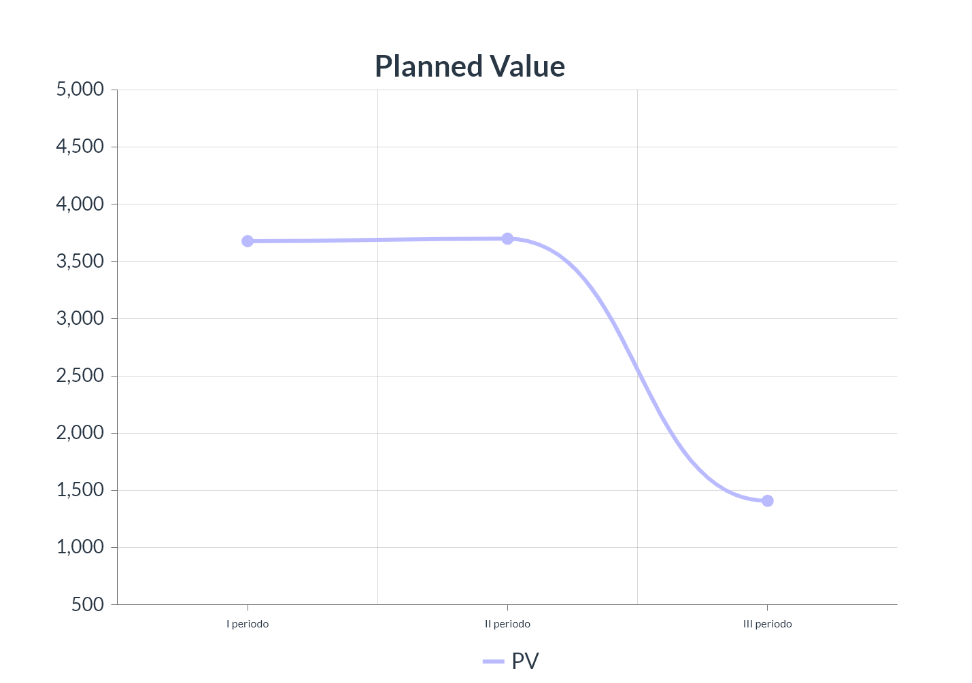
\includegraphics[width=10cm]{./res/images/PVGraph.png}
  \caption{Planned Value}
  \label{fig:Grafico Planned Value}
\end{figure}
\end{center}
\pagebreak
\paragraph{Actual Cost}
\begin{center}
\begin{figure}[H]
  \centering
  \renewcommand{\thefigure}{2}
  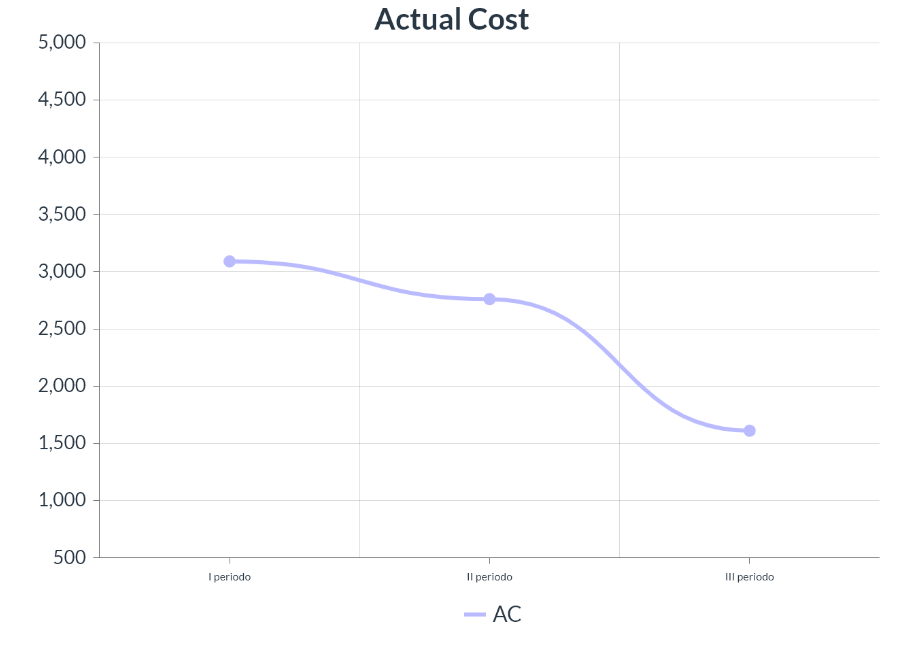
\includegraphics[width=10cm]{./res/images/ACGraph.png}
  \caption{Actual Cost}
  \label{fig:Grafico Actual Cost}
\end{figure}
\end{center}
\paragraph{Earned Value}
\begin{center}
\begin{figure}[H]
  \centering
  \renewcommand{\thefigure}{3}
  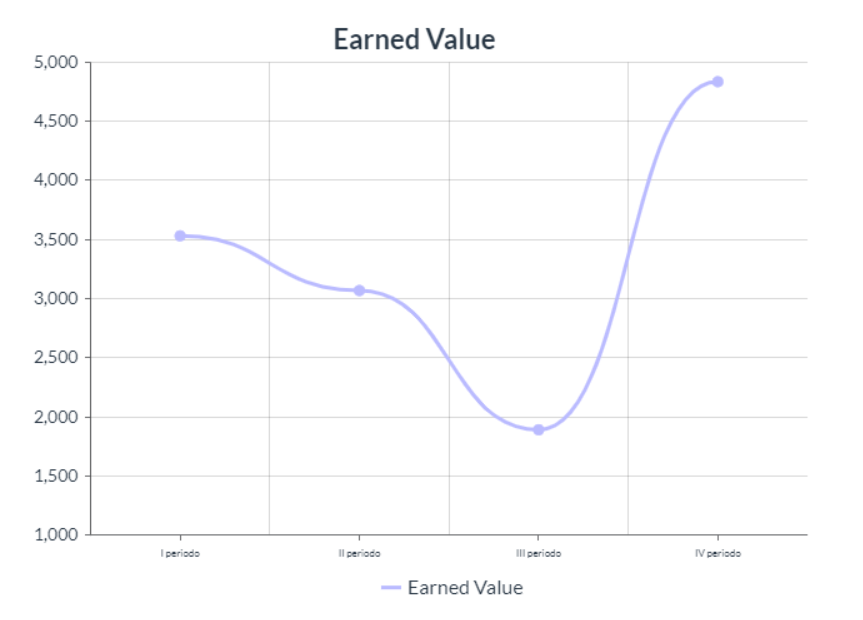
\includegraphics[width=10cm]{./res/images/EVGraph.png}
  \caption{Earned Value}
  \label{fig:Grafico Earned Value}
\end{figure}
\end{center}
\pagebreak
\paragraph{Cost Variance}
\begin{center}
\begin{figure}[H]
  \centering
  \renewcommand{\thefigure}{4}
  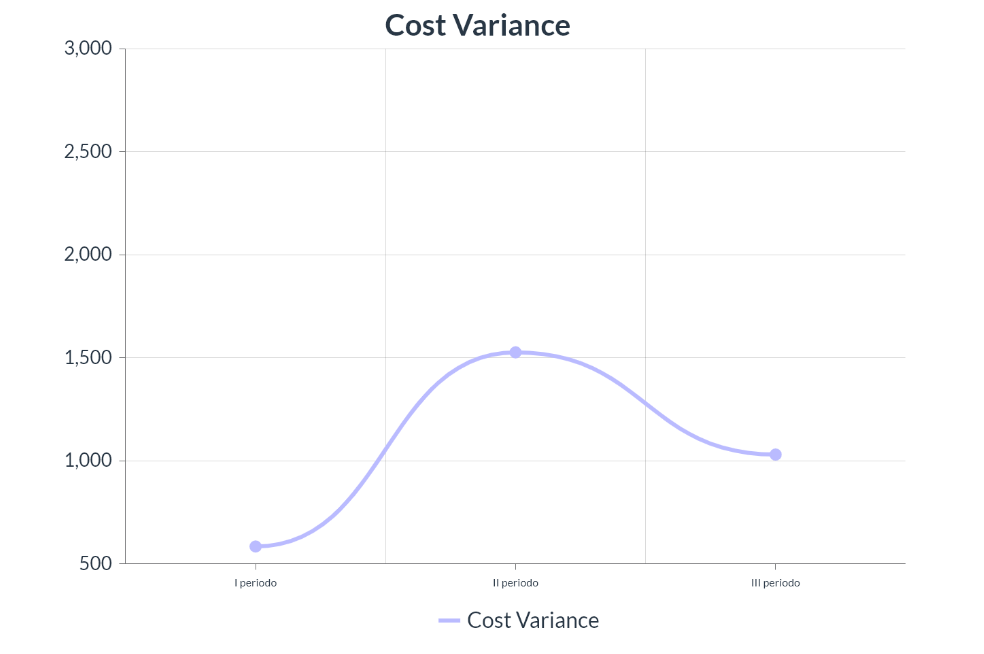
\includegraphics[width=10cm]{./res/images/CVGraph.png}
  \caption{Cost Variance}
  \label{fig:Grafico Cost Variance}
\end{figure}
\end{center}

\paragraph{Schedule Variance}
\begin{center}
\begin{figure}[H]
  \centering
  \renewcommand{\thefigure}{5}
  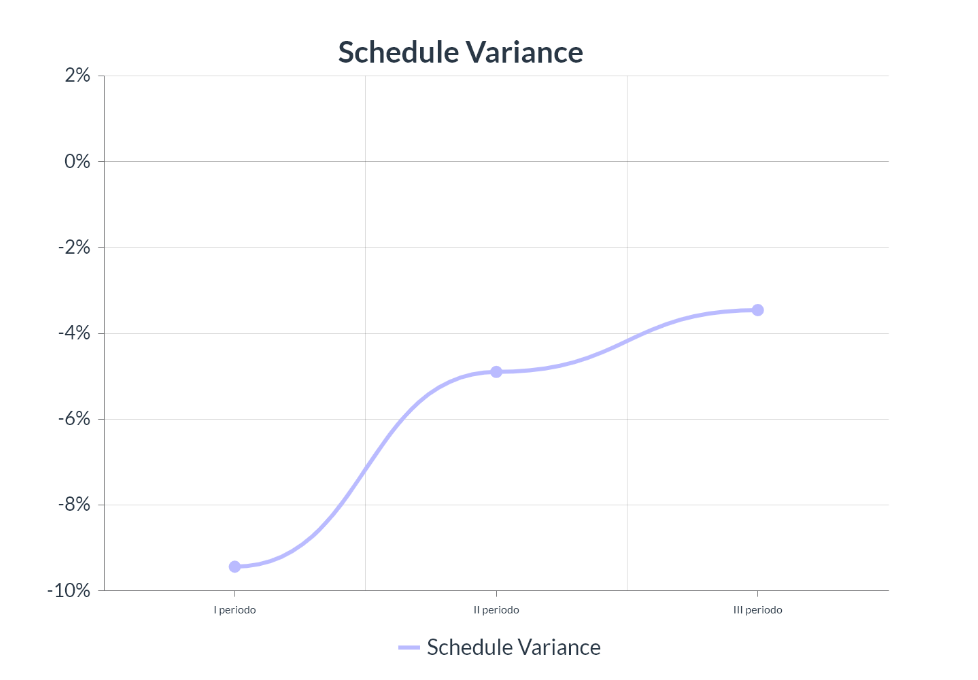
\includegraphics[width=10cm]{./res/images/SVGraph.png}
  \caption{Schedule Variance}
  \label{fig:Grafico Schedule Variance}
\end{figure}
\end{center}
\pagebreak
\paragraph{Budget Variance}
\begin{center}
\begin{figure}[H]
  \centering
  \renewcommand{\thefigure}{6}
  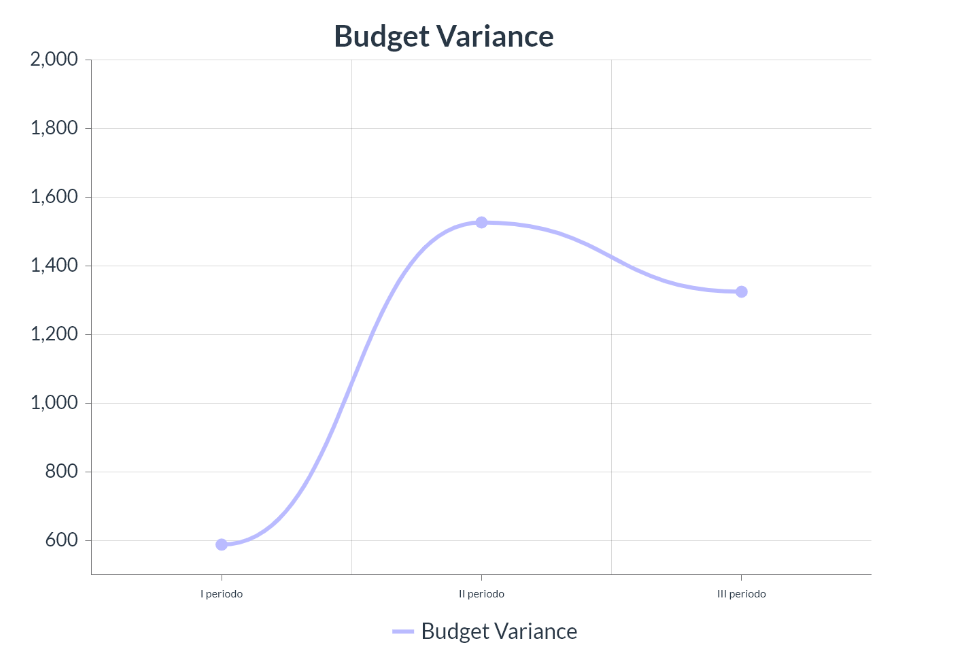
\includegraphics[width=10cm]{./res/images/BVGraph.png}
  \caption{Budget Variance}
  \label{fig:Grafico Budget Variance}
\end{figure}
\end{center}

\subsubsection{Indice di Gulpease}
\noindent Nella seguente tabella vengono riportati gli indici di Gulpease calcolati sulle ultime versioni dei seguenti documenti.\\
Per calcolare i seguenti valori non sono stati considerati: i changelog, la pagina di introduzione del documento, l'indice, tabelle con valori, intestazioni a piè di pagina, captions e la sezione di "Informazioni generali" nei verbali. Sono state incluse invece le colonne di tabelle contenenti descrizioni significative e gli elenchi puntati che contenevano frasi significative. 
\begin{longtable}{ 
		>{\centering}M{0.45\textwidth} 
		>{\centering}M{0.17\textwidth}
		>{\centering}M{0.25\textwidth} 
		}
	\rowcolorhead
	\headertitle{Documento} &
	\centering \headertitle{Valore} &	
	\headertitle{Esito} 
	\endfirsthead	
	\endhead
	
	\textit{Analisi dei Requisiti} & 80 & Superato\tabularnewline
	\textit{Glossario} & 72 & Superato\tabularnewline
	\textit{Norme di Progetto} & 74 & Superato\tabularnewline
	\textit{Piano di Progetto} & 63 & Superato\tabularnewline
	\textit{Piano di Qualifica} & 76 & Superato\tabularnewline
	\textit{Studio di Fattibilità} & 80 & Superato\tabularnewline
	VE 22-10-25 & 82 & Superato\tabularnewline
	VE 22-10-26 & 84 & Superato\tabularnewline
	VE 22-11-17	& 75 & Superato\tabularnewline
	VE 23-01-11	& 57 & Superato\tabularnewline
	VE 23-01-18	& 69 & Superato\tabularnewline
	VE 23-02-17 & 70 & Superato\tabularnewline
	VE 23-04-05 & 60 & Superato\tabularnewline
	VE 23-04-14 & 63 & Superato\tabularnewline
	VE 23-05-12 & 64 & Superato\tabularnewline
	VI 22-10-25 & 74 & Superato\tabularnewline
	VI 22-10-26 & 79 & Superato\tabularnewline
	VI 22-11-04 & 63 & Superato\tabularnewline
	VI 22-11-09 & 88 & Superato\tabularnewline
	VI 22-11-16 & 63 & Superato\tabularnewline
	VI 22-11-23 & 72 & Superato\tabularnewline
	VI 22-12-01 & 60 & Superato\tabularnewline
	VI 22-12-07 & 78 & Superato\tabularnewline
	VI 22-12-14 & 69 & Superato\tabularnewline
	VI 23-01-04 & 63 & Superato\tabularnewline
	VI 23-01-25 & 68 & Superato\tabularnewline
	VI 23-02-01 & 65 & Superato\tabularnewline
	VI 23-02-08 & 58 & Superato\tabularnewline
	VI 23-02-24 & 68 & Superato\tabularnewline
	VI 23-02-28 & 65 & Superato\tabularnewline
	VI 23-03-16 & 67 & Superato\tabularnewline
	VI 23-04-23 & 70 & Superato\tabularnewline
	VI 23-05-05 & 67 & Superato\tabularnewline
	
\end{longtable}

\begin{center}
\begin{figure}[H]
  \centering
  \renewcommand{\thefigure}{7}
  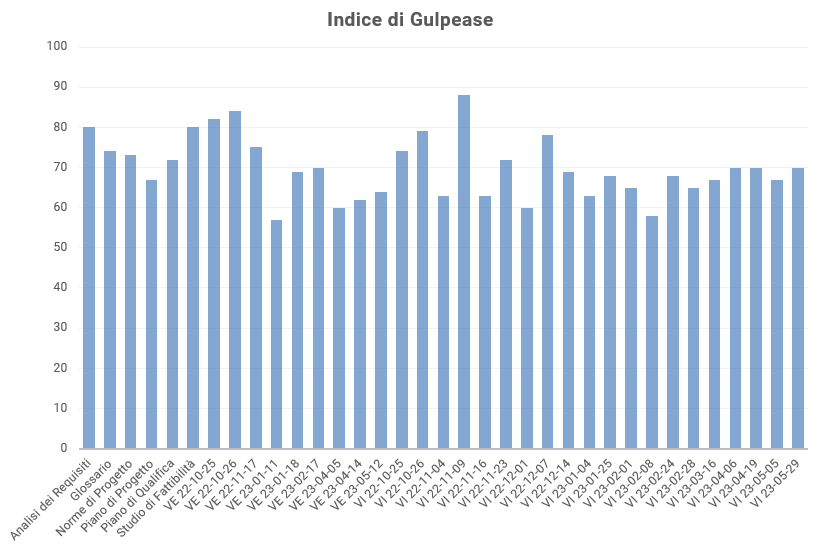
\includegraphics[width=10cm]{./res/images/GulpeaseGen.png}
  \caption{Indice di Gulpease dei documenti}
  \label{fig:Indice di Gulpease dei documenti}
\end{figure}
\end{center}
\pagebreak
\noindent Qui ora vengono riportati i grafici che analizzano l'andamento dell'indice di Gulpease di documenti in continua evoluzione.
\paragraph{Indice di Gulpease - \textit{Analisi dei Requisiti}}
\begin{center}
\begin{figure}[H]
  \centering
  \renewcommand{\thefigure}{8}
  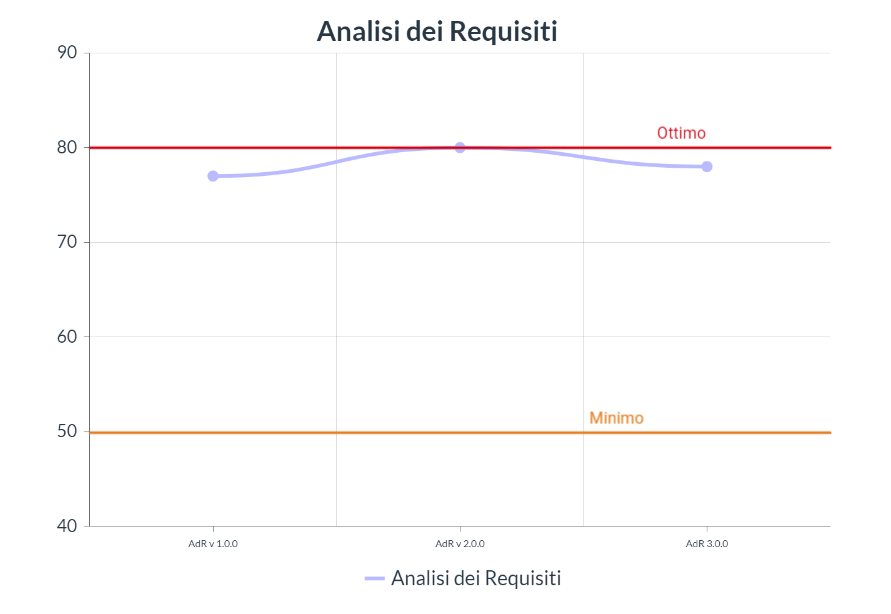
\includegraphics[width=10cm]{./res/images/AdRGraph.png}
  \caption{Indice di Gulpease - \textit{Analisi dei Requisiti}}
  \label{fig:Indice di Gulpease - Analisi dei Requisiti}
\end{figure}
\end{center}
\pagebreak
\paragraph{Indice di Gulpease - \textit{Norme di Progetto}}
\begin{center}
\begin{figure}[H]
  \centering
  \renewcommand{\thefigure}{9}
  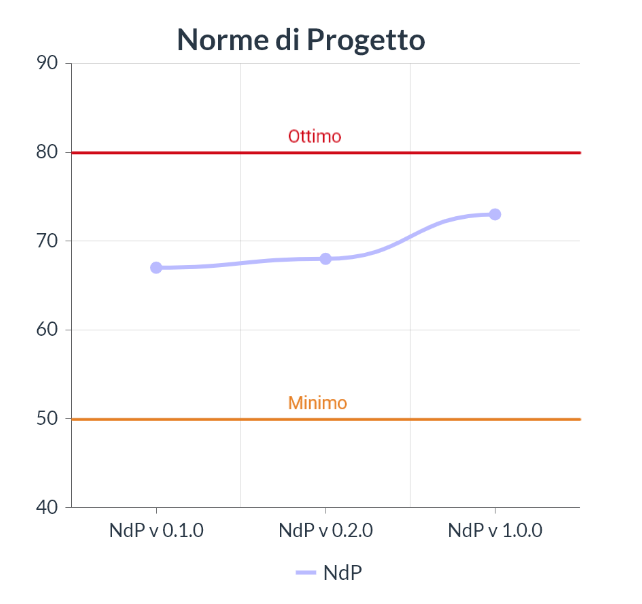
\includegraphics[width=10cm]{./res/images/NdPGraph.png}
  \caption{Indice di Gulpease - \textit{Norme di Progetto}}
  \label{fig:Indice di Gulpease - Norme di Progetto}
\end{figure}
\end{center}
\pagebreak
\paragraph{Indice di Gulpease - \textit{Piano di Progetto}}
\begin{center}
\begin{figure}[H]
  \centering
  \renewcommand{\thefigure}{10}
  \includegraphics[width=10cm]{./res/images/PdPGraph.png}
  \caption{Indice di Gulpease - \textit{Piano di Progetto}}
  \label{fig:Indice di Gulpease - Piano di Progetto}
\end{figure}
\end{center}
\pagebreak
\paragraph{Indice di Gulpease - \textit{Piano di Qualifica}}
\begin{center}
\begin{figure}[H]
  \centering
  \renewcommand{\thefigure}{11}
  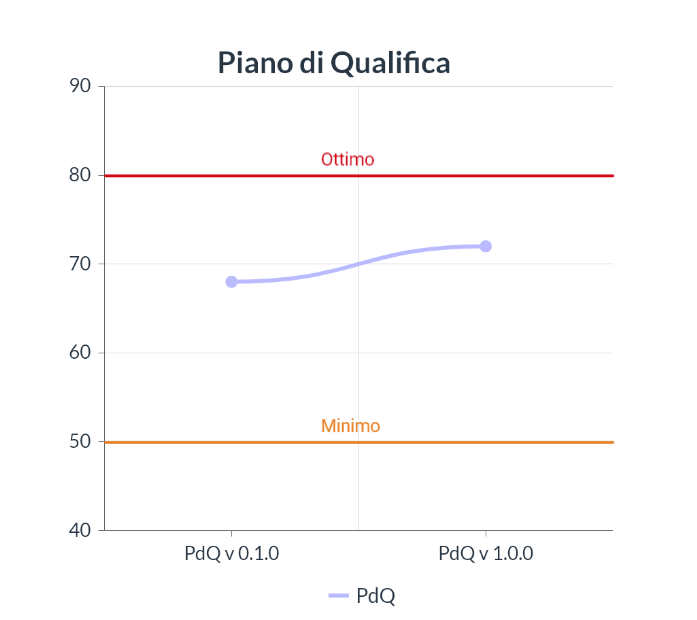
\includegraphics[width=10cm]{./res/images/PdQGraph.png}
  \caption{Indice di Gulpease - \textit{Piano di Qualifica}}
  \label{fig:Indice di Gulpease - Piano di Qualifica}
\end{figure}
\end{center}

\subsection{Verifica della qualità dei prodotti\textsubscript{g}}
In questa sezione vengono riportati i risultati dell'attività di verifica\textsubscript{g} effettuata relativa alla qualità del prodotto\textsubscript{g}, nel contesto del PoC\textsubscript{g}.\\
La metrica di Percentuale di requisiti soddisfatti non è stata testata in quanto non siamo ancora nella fase di Codifica.

\begin{longtable}{ 
		>{\centering}M{0.45\textwidth} 
		>{\centering}M{0.17\textwidth}
		>{\centering}M{0.25\textwidth} 
		}
	\rowcolorhead
	\headertitle{Metrica} &
	\centering \headertitle{Valore} &	
	\headertitle{Esito} 
	\endfirsthead	
	\endhead
	Percentuale di requisiti soddisfatti& - & Non testato\tabularnewline
	Densità di fallimenti durante l'esecuzione& 0\% & Superato\tabularnewline
	Tempo medio di risposta & minore di 1s & Superato\tabularnewline
	Tempo di caricamento& 7 secondi & Superato\tabularnewline
	Facilità di apprendimento& 90 secondi & Superato\tabularnewline
	Densità dei commenti & 15,93\% & Superato\tabularnewline
	Browser supportati & 100\% & Superato\tabularnewline
\end{longtable}
\noindent Nella seguente tabella è stata calcolata la Complessità Ciclomatica del PoC\textsubscript{g}.
\begin{longtable}{ 
		>{\centering}M{0.40\textwidth} 
		>{\centering}M{0.15\textwidth}
		>{\centering}M{0.20\textwidth}
		}
	\rowcolorhead
	\headertitle{Modulo} &
	\headertitle{Valore} &
	\headertitle{Esito} 	
	\endfirsthead	
	\endhead
	Player.js & 2 & Superato\tabularnewline
	Light.js & 1 & Superato\tabularnewline
	Product.js & 1 & Superato\tabularnewline
	Raycasting.js & 6 & Superato\tabularnewline
	Renderer.js & 2 & Superato\tabularnewline
	Showroom\_poc.js & 1 & Superato\tabularnewline
	Source\_loader.js & 2 & Superato\tabularnewline
	UI\_listeners.js & 1 & Superato\tabularnewline
	
\end{longtable}

Il PoC\textsubscript{g} è stato testato sui seguenti browser:
\begin{longtable}{ 
		>{\centering}M{0.45\textwidth} 
		>{\centering}M{0.25\textwidth} 
		}
	\rowcolorhead
	\headertitle{Browser} &
	\headertitle{Esito} 
	\endfirsthead	
	\endhead
	
	Google Chrome (versione $ \ge 110 $) & Supportato\tabularnewline
	Microsoft Edge (versione $ \ge 110 $) & Supportato\tabularnewline
	Mozilla Firefox (versione $ \ge 109 $) & Supportato\tabularnewline
	Safari (versione $ \ge 16 $) & Supportato\tabularnewline
	Opera (versione $ \ge 95 $) & Supportato\tabularnewline

\end{longtable}

\section{Specifica dei Test}
\begin{itemize}
\item Test di unità: vengono stabiliti durante la progettazione e servono per verificare le singole unità software;
\item Test di integrazione: vengono stabiliti durante la progettazione e servono per integrare il funzionamento di più unità;
\item Test di accettazione: vengono effettuati insieme al proponente\textsubscript{g} durante la fase di collaudo;
\item Test di sistema: vengono stabiliti durante l'\textit{Analisi dei Requisiti} e servono per accertare la copertura dei requisiti software definiti nel documento di \textit{Analisi dei Requisiti}.
\end{itemize}
Gli acronimi utilizzati in questo documento per identificare i test sono specificati dettagliatamente nel documento di \textit{Norme di Progetto}.
In questa sezione vengono utilizzate le seguenti sigle per lo stato di ogni test:
\begin{itemize}
\item \textbf{S}: test superato
\item \textbf{N}: test non implementato
\end{itemize}

\subsection{Test di unità}
Per garantire il funzionamento dei singoli componenti che possono lavorare in maniera autonoma senza bisogno di dipendenze abbiamo effettuato questi test. Non abbiamo ritenuto necessario testare componenti o parti di componenti che:
\begin{itemize}
	\item Utilizzavano funzionalità già assodate e documentate;
	\item Componenti che raggruppavano altri componenti.
\end{itemize} 
\begin{longtable}{
		>{\centering}M{0.20\textwidth}
		>{\centering}M{0.35\textwidth}	 
		>{\centering}M{0.20\textwidth} 
		}
	\rowcolorhead
	\headertitle{Test} &
	\centering \headertitle{Descrizione} &	
	\headertitle{Stato} 
	\endfirsthead	
	\endhead
TU1 & Si verifichi che la posizione del player cambi quando utilizza i tasti di movimento & S\tabularnewline
TU2 & Si verifichi che la rotazione del player cambi quando muove la visuale col mouse & S\tabularnewline
TU3 & Si verifichi che avvenga il cambiamento colore ad un oggetto interagibile & S\tabularnewline
TU4 & Si verifichi la funzionalità dell’aggiunta all’array che rappresenta gli oggetti nel carrello e l’incremento del costo totale & S\tabularnewline
TU5 & Si verifichi che la funzionalità di aggiungere un oggetto al carrello funzioni solo con oggetti validi & S\tabularnewline
TU6 & Si verifichi la possibilità di utilizzare i selettori Redux per reperire l’array logico del carrello e il costo totale & S\tabularnewline
TU7 & Si verifichi la funzionalità della rimozione totale dall’array del carrello & S\tabularnewline
TU8 & Si verifichi che la funzionalità di rimozione totale dell’array carrello funzioni anche se il carrello è vuoto & S\tabularnewline
TU9 & Si verifichi la funzionalità di eliminazione singola dal carrello & S\tabularnewline
TU10 & Si verifichi che l’eliminazione singola funziona solo con oggetti realmente presenti nell’array carrello & S\tabularnewline
TU11 & Si verifichi che il raycaster funzioni & S\tabularnewline
TU12 & Si verifichi che funzioni la possibilità di aggiungere quantità di un oggetto selezionato & S\tabularnewline
TU13 & Si verifichi che funzioni la possibilità di diminuire quantità di un oggetto selezionato & S\tabularnewline
\end{longtable}

\subsection{Test di integrazione}
Per assicurare che ogni componente lavori correttamente con gli altri componenti, il gruppo ha deciso di effettuare i seguenti Test di Integrazione.
\begin{longtable}{
		>{\centering}M{0.20\textwidth}
		>{\centering}M{0.35\textwidth}	 
		>{\centering}M{0.20\textwidth} 
		}
	\rowcolorhead
	\headertitle{Test} &
	\centering \headertitle{Descrizione} &	
	\headertitle{Stato} 
	\endfirsthead	
	\endhead
TI1 & Si verifichi che la modifica di cambiamento colore venga apportata ad un oggetto esempio nel file JSON contenente i prodotti interagibili & S\tabularnewline
TI2 & Si verifichi che un elemento nel carrello , se eliminato singolarmente, scompaia dal componente Cart e anche dall’array logico del carrello & S\tabularnewline
TI3 & Si verifichi che il bottone “Remove all” funzioni rimuovendo sia da Cart che da cartSlice tutti gli oggetti & S\tabularnewline
TI4 & Si verifichi che il bottone “Remove all” funzioni anche se il carrello è vuoto & S\tabularnewline
TI5 & Si verifichi che il cambio di colore nella Sidebar venga salvato & S\tabularnewline
TI6 & Si verifichi che il colore ritorni a standard se viene deselezionata una modifica di colore & S\tabularnewline
TI7 & Si verifichi che venga aggiunto un oggetto al carrello dalla sidebar & S\tabularnewline
TI8 & Si verifichi che venga aggiunta la quantità selezionata di un oggetto già presente nel carrello & S\tabularnewline
\end{longtable}
\subsection{Test di accettazione}
Questi test verranno stabiliti durante la fase di Collaudo.

\subsection{Test di sistema}
Per assicurare che vengano rispettati i requisiti concordati nel documento di \textit{Analisi dei Requisiti}, vengono eseguiti i seguenti test di sistema.
\begin{longtable}{
		>{\centering}M{0.20\textwidth}
		>{\centering}M{0.35\textwidth}	 
		>{\centering}M{0.20\textwidth} 
		}
	\rowcolorhead
	\headertitle{Test} &
	\centering \headertitle{Descrizione} &	
	\headertitle{Stato} 
	\endfirsthead	
	\endhead
TSRF1 & Si verifica\textsubscript{g} che l'utente possa aggiungere, l'oggetto con cui sta interagendo, nel carrello & S \tabularnewline
TSRF2 & Si verifica\textsubscript{g} che l'utente possa visualizzare il contenuto del carrello & S \tabularnewline
TSRF2.1 & Si verifica\textsubscript{g} che l'utente possa visualizzare la lista degli oggetti presenti nel carrello & S \tabularnewline
TSRF2.1.1 & Si verifica\textsubscript{g} che l'utente possa interagire con un oggetto nel carrello & S \tabularnewline
TSRF2.1.1.1 & Si verifica\textsubscript{g} che l'utente possa visualizzare la caratteristica del nome di ogni oggetto presente nella lista degli oggetti presenti nel carrello & S \tabularnewline
TSRF2.1.1.2 & Si verifica\textsubscript{g} che l'utente possa visualizzare la caratteristica del costo di ogni oggetto presente nella lista degli oggetti presenti nel carrello & S \tabularnewline
TSRF2.1.1.3 & Si verifica\textsubscript{g} che l'utente possa visualizzare la caratteristica della quantità di ogni oggetto presente nella lista degli oggetti presenti nel carrello & S \tabularnewline
TSRF2.2 & Si verifica\textsubscript{g} che l'utente possa visualizzare il costo totale degli oggetti che ha inserito nel carrello & S \tabularnewline
TSRF3 & Si verifica\textsubscript{g} che l'utente abbia la possibilità di rimuovere tutti gli oggetti dal carrello & S \tabularnewline
TSRF4 & Si verifica\textsubscript{g} che l'utente abbia la possibilità di rimuovere un singolo oggetto dal carrello & S \tabularnewline
TSRF5 & Si verifica\textsubscript{g} che l'utente possa muoversi in maniera direzionale & S \tabularnewline
TSRF5.1 & Si verifica\textsubscript{g} che l'utente possa compiere movimenti direzionali nell'asse X & S \tabularnewline
TSRF5.2 & Si verifica\textsubscript{g} che l'utente possa compiere movimenti direzionali nell'asse Y & S \tabularnewline
TSRF5.3 & Si verifica\textsubscript{g} che l'utente possa compiere movimenti direzionali nell'asse Z & S \tabularnewline
TSRF6 & Si verifica\textsubscript{g} che l'utente possa compiere spostamenti di camera & S \tabularnewline
TSRF6.1 & Si verifica\textsubscript{g} che l'utente possa compiere spostamenti di camera nell'asse X & S \tabularnewline
TSRF6.2 & Si verifica\textsubscript{g} che l'utente possa compiere spostamenti di camera nell'asse Y & S \tabularnewline
TSRF7 & Si verifica\textsubscript{g} che l'utente possa modificare la combinazione dei colori di un oggetto & S \tabularnewline
TSRF8 & Si verifica\textsubscript{g} che l'utente venga notificato in caso non fosse possibile modificare un oggetto & S \tabularnewline
TSRF9 & Si verifica\textsubscript{g} che l'utente possa visualizzare la lista degli oggetti della stanza in cui si trova & N \tabularnewline
TSRF9.1 & Si verifica\textsubscript{g} che l'utente possa visualizzare un singolo oggetto nella lista degli oggetti della stanza in cui si trova & N \tabularnewline
TSRF9.1.1 & Si verifica\textsubscript{g} che l'utente possa visualizzare la caratteristica del nome di ogni oggetto della lista degli oggetti della stanza in cui si trova & N \tabularnewline
TSRF10 & Si verifica\textsubscript{g} che l'utente possa visualizzare tutti i dettagli di un oggetto selezionato & S \tabularnewline
TSRF11 & Si verifica\textsubscript{g} che l'utente abbia la possibilità di riposizionarsi vicino ad un oggetto nella stanza in cui si trova & N \tabularnewline
TSRF12 & Si verifica\textsubscript{g} che l'utente possa riposizionarsi in una stanza da lui selezionata & N \tabularnewline
TSRF13 & Si verifica\textsubscript{g} che l'utente venga notificato in caso il riposizionamento in una stanza non sia possibile & N \tabularnewline
TSRF14 & Si verifica\textsubscript{g} che l'utente venga notificato in caso il riposizionamento in prossimità di un oggetto selezionato non sia concesso & N \tabularnewline
TSRF15 & Si verifica\textsubscript{g} che l'utente possa visualizzare la lista delle stanze & N \tabularnewline
TSRF15.1 & Si verifica\textsubscript{g} che l'utente possa visualizzare una singola stanza dalla lista delle stanze & N \tabularnewline
TSRF15.1.1 & Si verifica\textsubscript{g} che l'utente possa visualizzare la caratteristica del nome di ogni stanza dalla lista delle stanze & N \tabularnewline
TSRF15.1.2 & Si verifica\textsubscript{g} che l'utente possa visualizzare la caratteristica della tipologia di oggetti presenti in ogni stanza nella lista delle stanze & N \tabularnewline
TSRF16 & Si verifica\textsubscript{g} che l'utente possa riposizionare un oggetto presente nella stanza in cui si trova & N \tabularnewline
TSRF17 & Si verifica\textsubscript{g} che l'utente non possa riposizionare un oggetto in una coordinata non legittima & N \tabularnewline
TSRF18 & Si verifica\textsubscript{g} che l'utente sia in grado ad illuminare l'ambiente davanti a lui & S \tabularnewline
TSRF19 & Si verifica\textsubscript{g} che l'utente venga notificato se il contenuto del carrello è vuoto & S \tabularnewline
TSRF20 & Si verifica\textsubscript{g} che l'utente possa visualizzare un oggetto illuminato & S \tabularnewline
\end{longtable}

\subsection{Tracciamento dei test}
\subsubsection{Test di Sistema - Requisiti}
\begin{longtable}{
		>{\centering}M{0.25\textwidth}
		>{\centering}M{0.25\textwidth}	 
		}
	\rowcolorhead
	\headertitle{Test di sistema} &
	\headertitle{Requisiti}
	\endfirsthead	
	\endhead
TSRF1 & RF1\tabularnewline
TSRF2 & RF2\tabularnewline
TSRF2.1 & RF2.1\tabularnewline
TSRF2.1.1 & RF2.1.1\tabularnewline
TSRF2.1.1.1 & RF2.1.1.1\tabularnewline
TSRF2.1.1.2 & RF2.1.1.2\tabularnewline
TSRF2.1.1.3 & RF2.1.1.3\tabularnewline
TSRF2.2 & RF2.2\tabularnewline
TSRF3 & RF3\tabularnewline
TSRF4 & RF4\tabularnewline
TSRF5 & RF5\tabularnewline
TSRF5.1 & RF5.1\tabularnewline
TSRF5.2 & RF5.2\tabularnewline
TSRF5.3 & RF5.3\tabularnewline
TSRF6 & RF6\tabularnewline
TSRF7 & RF7\tabularnewline
TSRF8 & RF8\tabularnewline
TSRF9 & RF9\tabularnewline
TSRF9.1 & RF9.1\tabularnewline
TSRF9.1.1 & RF9.1.1\tabularnewline
TSRF10 & RF10\tabularnewline
TSRF11 & RF11\tabularnewline
TSRF12 & RF12\tabularnewline
TSRF13 & RF13\tabularnewline
TSRF14 & RF14\tabularnewline
TSRF15 & RF15\tabularnewline
TSRF15.1 & RF5.1\tabularnewline
TSRF15.1.1 & RF15.1.1\tabularnewline
TSRF15.1.2 & RF15.1.2\tabularnewline
TSRF16 & RF16\tabularnewline
TSRF17 & RF17\tabularnewline
TSRF18 & RF18\tabularnewline
TSRF19 & RF19\tabularnewline
TSRF20 & RF20\tabularnewline

\end{longtable}

\subsubsection{Test di Unità - File di Test}
\begin{longtable}{
		>{\centering}M{0.10\textwidth}
		>{\centering}M{0.30\textwidth}
		>{\centering}M{0.45\textwidth}	 
		}
	\rowcolorhead
	\headertitle{Test} &
	\centering \headertitle{File di test} &	
	\centering \headertitle{Nome test} 
	\endfirsthead	
	\endhead
TU1 & \_\_test\_\_/playerSlice.test.js & it(’should set the player position’)\{ … \}\tabularnewline
TU2 & \_\_test\_\_/playerSlice.test.js & it(’should set the player rotation’)\{ … \}\tabularnewline
TU3 & \_\_test\_\_/productSlice.test.js & it('Should change color to the product in example')\{ … \}\tabularnewline
TU4 & \_\_test\_\_/cartSlice.test.js & it('Should add an item to the array (that represents the logic of the cart) of the slice and increment the totalCost’)\{ … \}\tabularnewline
TU5 & \_\_test\_\_/cartSlice.test.js & it('Should not be able to add this item’) \{ … \}\tabularnewline
TU6 & \_\_test\_\_/cartSlice.test.js & it('Should be able to use the cartItems selector and the totalCost selector’)\{ … \}\tabularnewline
TU7 & \_\_test\_\_/cartSlice.test.js & it('Should remove all the item in the cart')\{ … \}\tabularnewline
TU8 & \_\_test\_\_/cartSlice.test.js & it('Should remove all the items even if the cart is empty’)\{ … \}\tabularnewline
TU9 & \_\_test\_\_/cartSlice.test.js & it('Should remove the item in example’)\{ … \}\tabularnewline
TU10 & \_\_test\_\_/cartSlice.test.js & it('Should be able to work even if the item provided do not exist in the cart’)\{ … \}\tabularnewline
TU11 & \_\_test\_\_/useRaycasterLogic.test.js & it('should update intersects when mouse moves’)\{ … \}\tabularnewline
TU12 & \_\_test\_\_/productSidebar.test.js & it('Should add more then one quantity of the item selected’)\{ … \}\tabularnewline
TU13 & \_\_test\_\_/productSidebar.test.js & it('Should decrease of one the quantity of the item’)\{ … \}\tabularnewline
\end{longtable}

\subsubsection{Test di Integrità - File di Test}
\begin{longtable}{
		>{\centering}M{0.10\textwidth}
		>{\centering}M{0.30\textwidth}
		>{\centering}M{0.45\textwidth}	 
		}
	\rowcolorhead
	\headertitle{Test} &
	\centering \headertitle{File di test} &	
	\centering \headertitle{Nome test} 
	\endfirsthead	
	\endhead
TI1 & \_\_test\_\_/productSlice.test.js & it('Should change color to the product with the ID=1 imported from the JSON file’)\{ … \} \tabularnewline
TI2 & \_\_test\_\_/cart.test.js & it('Should stop rendering item in cart when clicking "X" button’)\{ … \}\tabularnewline
TI3 & \_\_test\_\_/cart.test.js & it('Should stop rendering all items in cart when clicking "Remove all" button’)\{ … \}\tabularnewline
TI4 & \_\_test\_\_/cart.test.js & it('Should try to remove the items and work even if cart is empty’)\{ … \}\tabularnewline
TI5	& \_\_test\_\_/productSidebar.test.js & it('Should change the variable selectedColor to the product in example’)\{ … \}\tabularnewline
TI6 & \_\_test\_\_/productSidebar.test.js & it('Should remove the selected color if the button with the current color is pressed, putting the standard color to the item’)\{ … \}\tabularnewline
TI7 & \_\_test\_\_/productSidebar.test.js & it('Should add an item to the cart’)\{ … \}\tabularnewline
TI8 & \_\_test\_\_/productSidebar.test.js & it('Should add more than one quantity of the item to the cart, testing also if it adds the quantity to the item that is already in the cart’)\{ … \}\tabularnewline
\end{longtable}
\pagebreak

\end{document}
